\documentclass[a4paper]{article}
\usepackage[letterpaper, margin=1in]{geometry}  	% use "amsart" instead of "article" for AMSLaTeX format          
\geometry{letterpaper}                   		% ... or a4paper or a5paper or ... 
\usepackage{listings,graphicx,amsmath, amssymb, amsfonts, amsthm,tikz,hyperref,fullpage,setspace,enumerate,mathtools,arydshln} 

\title{A.I. Midterm}
\author{Helen Ngo}
\date{\today}							% Activate to display a given date or no date

\begin{document}
\maketitle
\section{Classification Task} 

Compare two algorithms on a classification task: the Pocket algorithm (designed for classification), and linear regression (not designed for classification). For linear regression, after learning the weights $\textbf{w}$; we use $h(\textbf{x}) = \textrm{sign}(\textbf{w}^T\textbf{x})$ to classify $\textbf{x}$. For the dataset, start by using the given code. Then create another dataset using the same methods as above, which we will use to estimate $E_{out}$. Try the following three approaches using multiple randomized experiments and explain which works best in terms of both $E_{out}$ and the amount of computation required. 

\begin{enumerate}[(a)]
\item The Pocket algorithm, starting from $\textbf{w} = 0$.
\item Linear regression (applied as a classification method).
\item The Pocket algorithm, starting from the solution given by linear regression.
\end{enumerate}

\begin{doublespace}

\subsection{Classifying between 0 and Everything Else}

When producing the dataset from ``features.csv" where $0$ is classified against everything else, we get the plot on the next page. Note that zero was assigned the positive class in blue. For this linearly inseparable dataset it took:

\begin{enumerate}[(a)]
\item The Pocket algorithm took $1223$ iterations and approximately 4 minutes to converge, with $E_{out} \approx 0.1078$.
\item Linear regression produced a hypothesis with $E_{out} \approx 0.1086$ in about 0.5 minutes.
\item The Pocket algorithm starting from a linear regression solution took $864$ iterations and ~2.5 minutes to converge. The $E_{out} \approx 0.1059$.
\end{enumerate}

It should be noted that convergence is either no classification error, more than 500 iterations with the same optimal hypothesis, or more than ten thousand total iterations, which can be seen in the pla function.

\lstinputlisting[language=Python, firstline=121, lastline=139,frame=single]{midterm.py}

\begin{center}
	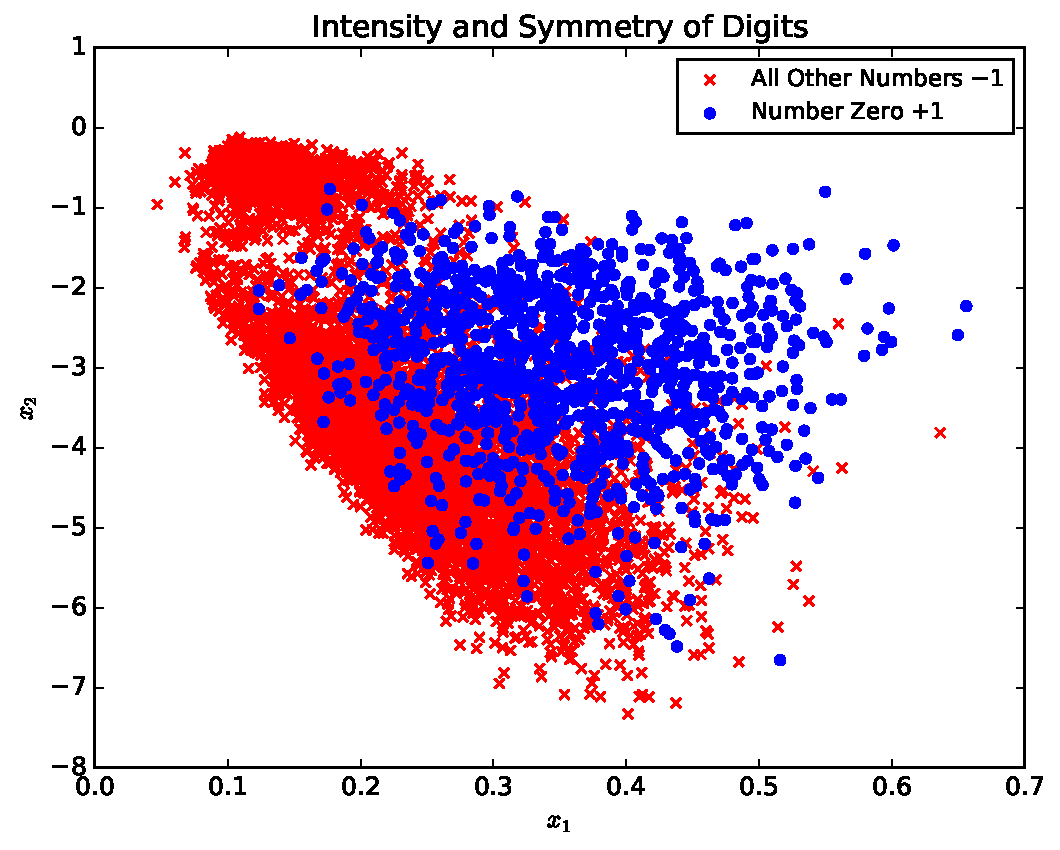
\includegraphics[scale =0.65]{By_Zero/midterm_plot.pdf}
\end{center}

\newpage

The Pocket algorithm starting from a linear regression, algorithm (c), had the lowest classification error at $E_{out} \approx 0.1059$, but it was only better than the hypothesis produced by linear regression, algorithm (b), which had a classification error of $E_{out} \approx 0.1086$. Algorithm (c) was less than $1\%$ better at classifying the negative and positive classes but took approximately $5$ times the amount of time as algorithm (b). The Pocket algorithm, algorithm (a), had the longest computing time and only classified $0.0010$ more points better than linear regression.

\subsection{Classifying between 1 and Everything Else}

When producing the dataset from ``features.csv" where $1$ is classified against everything else, we get the plot below. Note that zero was assigned the positive class in blue.

\begin{center}
	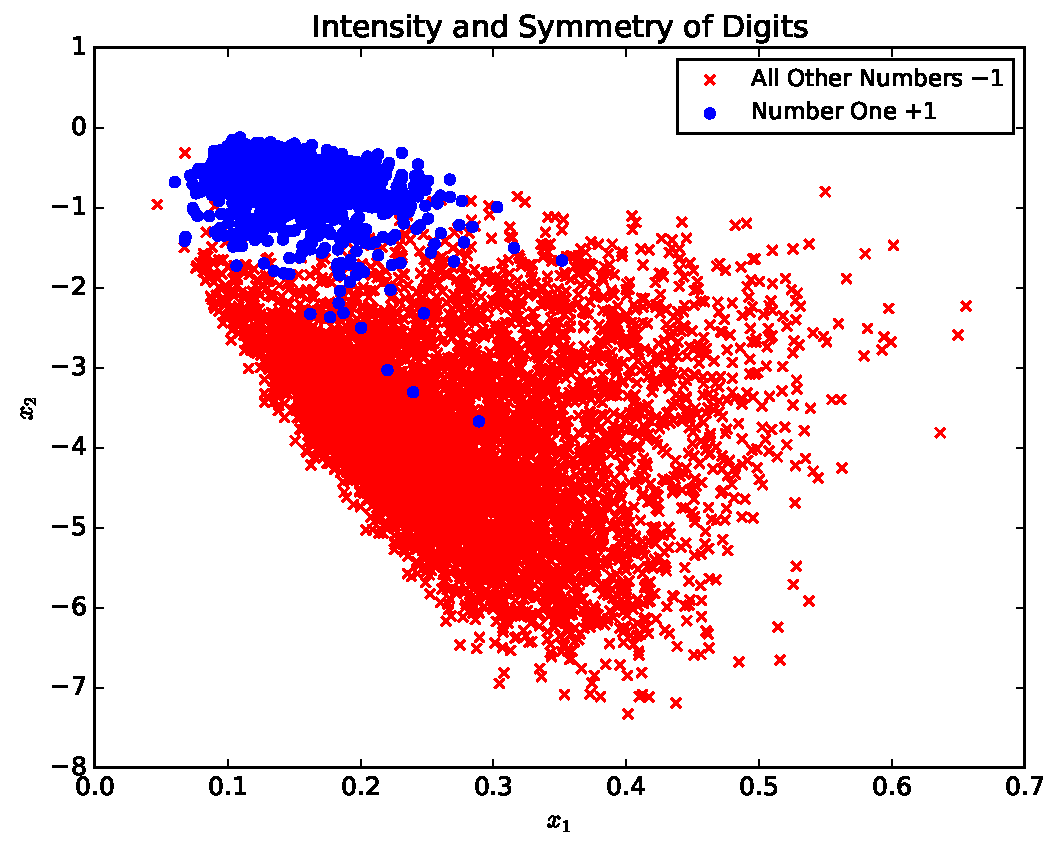
\includegraphics[scale =0.65]{By_One/midterm_plot.pdf}
\end{center}

For this linearly inseparable dataset it took:

\begin{enumerate}[(a)]
\item The Pocket algorithm took $1115$ iterations and approximately 4 minutes to converge, with $E_{out} \approx 0.0121$.
\item Linear regression produced a hypothesis with $E_{out} \approx 0.0152$ in about 0.5 minutes.
\item The Pocket algorithm starting from a linear regression solution took $1151$ iterations and ~5 minutes to converge. The $E_{out} \approx 0.0121$.
\end{enumerate}

For classifying between 1 and everything else, the algorithm (a) and algorithm (c) has the same classification error, $E_{out} \approx 0.0121$, but algorithm (c) took more iterations and about 1 more minute to converge. Once again, linear regression misclassified less than $1\%$ more than the pocket algorithms, and only took about significantly less time than both algorithms (a) and (c).

\subsection{Conclusion}

The Pocket algorithm starting from a liner regression solution consistently produced the lowest $E_{out}$ and could take from approximately the minimum number of iterations for convergence to the same amount as the normal Pocket algorithm. Therefore the number of computation is either similar to algorithm (a) or less, but the $E_{out}$ will always be the lowest (possibly tied). Linear regression for these datasets produced a minusculy higher $E_{out}$, but at significantly less computing time. If you need to minimize the the $E_{out}$, the Pocket algorithm starting from a linear regression solution would be preferred, but for a computationally efficient overview, linear regression will probably do fine.

\section{Problem 2.12}
For an $\mathcal{H}$ with $d_{vc} = 10$, what sample size do you need (as prescribed by the generalized bound) to have a $95\%$ confidence that your generalization error is at most 0.05?

\subsection{Iterative Method}
Using equation (2.13), we need
\[N \geq \frac{8}{0.05^2} \ln \left(\frac{4(2N)^{10}+4}{0.05}\right),\]
where $N \in \mathbb{Z}$. We know that the equation converges as an iterative method, where each iteration
\[N_i \geq \frac{8}{0.05^2} \ln \left(\frac{4(2N_{i-1})^{10}+4}{0.05}\right).\]
We know that the equation has converged when $N_i/N_{i-1} = 1$. 

\newpage

The python code for the equation as an iterative method:

\lstinputlisting[language=Python, frame=single]{gen_error.py}

Running this python code we get $N = 452957$. Putting this into equation (2.13), we get 
\[452957 \geq \frac{8}{0.05^2} \ln \left(\frac{4(2(452957))^{10}+4}{0.05}\right).\]
Thus $N = 452957$.

\newpage

\section{Drawing of the Professor}
\end{doublespace}
\end{document}  